\documentclass[11pt,a4paper]{article}
\usepackage[margin=2.5cm]{geometry}
\usepackage{mathptmx}
\usepackage[T1]{fontenc}
\usepackage{amsmath}
\usepackage{booktabs}
\usepackage{float}
\usepackage{graphicx}
\usepackage[dvipsnames]{xcolor}
\usepackage{setspace}
\usepackage{caption}
\usepackage[colorlinks=true,linkcolor=black,urlcolor=blue]{hyperref}
\setstretch{1.12}
\captionsetup{font=small,labelfont=bf}

% Auto-generated by corrected.py - do not edit by hand.
\newcommand{\SailFour}{0.3}
\newcommand{\SailSix}{2.2}
\newcommand{\SailEight}{16.0}
\newcommand{\EDTSix}{45.4}
\newcommand{\PropSix}{174.8}
\newcommand{\EDTover}{82}
\newcommand{\PROPover}{599}
\newcommand{\MeanSix}{74.1}
\newcommand{\EDTcross}{540}
\newcommand{\PROPcross}{405}
\newcommand{\KsensSail}{0.3}
\newcommand{\KsensEDT}{6.8}
\newcommand{\KsensProp}{26}
\newcommand{\ValLo}{7}
\newcommand{\ValHi}{13}
\newcommand{\ValMAPE}{900}
\newcommand{\ValEstFour}{67}
\newcommand{\ValAauThree}{196}
\newcommand{\ValPerseus}{176}
\newcommand{\ValModelGRB}{52.7}
\newcommand{\ValModelDhabi}{17.9}
\newcommand{\ValModelEst}{66.6}
\newcommand{\ValModelAau}{196.1}
\newcommand{\ValModelPerseus}{176.0}
\newcommand{\DensLo}{1.4}
\newcommand{\DensHi}{4.3}


% Highlights items that still need the original data / a decision. Delete before submission.
\newcommand{\pending}[1]{\par\medskip\noindent\fcolorbox{red}{red!6}{\parbox{\dimexpr\linewidth-2\fboxsep-2\fboxrule}{\small\color{red!70!black}\textbf{PENDING:} #1}}\par\medskip}
\newcommand{\pendinginline}[1]{{\color{red!70!black}\textbf{[#1]}}}

\title{\bfseries Quantifying the Deorbit Time of CubeSats:\\ A Comparative Analysis of Drag Sails, Propulsion, and Tethers\\[4pt]\large Corrected version}
\author{Aisha Shermatova\\{\small Kyrgyz-Turkish Anatolian High School for Girls, Bishkek, Kyrgyzstan}}
\date{}

\begin{document}
\maketitle

\begin{abstract}
The growing number of CubeSat launches in Low Earth Orbit (LEO) increases concerns about space debris and the need to follow the 25-year deorbit rule. Although several deorbit methods are available, there are few simple and student-friendly models to compare their performance. In this study, we created a straightforward orbital decay model to estimate and compare how long it takes a standard 3U CubeSat to deorbit using three technologies: drag sails, electrodynamic tethers, and cold-gas propulsion systems. The model uses the satellite's area-to-mass ratio and a simplified representation of how atmospheric density decreases with altitude.
We compared the model with the observed lifetimes of five CubeSats and found that it overestimates the lifetimes of satellites that have already decayed by a factor of roughly \ValLo--\ValHi; absolute deorbit times should therefore be read as upper estimates, while the relative comparison, which depends only on the area-to-mass ratio, is unaffected. Results show that a drag sail offers the fastest deorbit across altitudes from 400--800\,km, meeting the 25-year guideline in about \SailSix{} years from 600\,km. In comparison, electrodynamic tethers (when modeled conservatively as passive devices) and propulsion systems (without active deorbiting) took much longer, exceeding the guideline under the model's assumptions. These findings suggest that drag sails offer the shortest passive deorbit time for typical CubeSat missions; reliability of deployment, cost and regulatory acceptance were not modeled. This work gives student and small-team developers an easy-to-use, quantitative tool to choose deorbit methods, emphasizing the value of planning for sustainable satellite disposal from the start.
\end{abstract}

\section{Introduction}
The advent of CubeSats has democratized access to space, enabling universities, research groups, and small organizations to conduct educational and scientific missions with low-cost, modular platforms~\cite{villela}. However, the rapid proliferation of these satellites in Low Earth Orbit (LEO) has intensified concerns regarding space debris sustainability~\cite{esa2025}. Current estimates indicate that Earth orbit contains more than a million debris objects larger than 1\,cm, with impact velocities capable of damaging or destroying operational satellites~\cite{esa2025}. This environment creates long-term risks for space operations and increases the probability of self-sustaining collision cascades, known as the Kessler Syndrome~\cite{kessler}.

To mitigate these risks, international space debris mitigation guidelines, such as the 25-year rule, recommend that satellites be designed to re-enter Earth's atmosphere within 25 years of mission completion~\cite{iadc}. While larger satellites often employ propulsion systems for controlled deorbiting, most CubeSats lack the mass, volume, and power resources for such conventional systems~\cite{lemmer,selva}. Consequently, many CubeSats risk remaining in orbit long after their operational life, potentially violating mitigation standards and exacerbating orbital congestion.

Several dedicated deorbit technologies have been developed for small satellites to address this challenge, including drag sails, electrodynamic tethers, and miniature propulsion modules~\cite{sanchez,altaf}. Drag sails are passive devices that increase a satellite's cross-sectional area to enhance atmospheric drag~\cite{zhang,chen}. Electrodynamic tethers generate a Lorentz force through interaction with Earth's magnetic field to provide active or passive deceleration~\cite{forward,ohkawa,sarego}. Propulsion systems can perform targeted deorbit burns but are often resource-intensive. While previous studies describe the mechanics and advantages of these systems, most comparisons are qualitative or rely on complex simulation tools beyond the reach of student and small-scale projects~\cite{nasa2022,altaf}. A clear gap exists for simple, consistent, and student-accessible quantitative models that directly compare deorbit timelines for different technologies under unified assumptions.

This paper fills a critical gap by presenting a unified, first-order comparative framework that enables transparent cross-technology evaluation using only the area-to-mass ratio and an exponential atmospheric density approximation. Unlike complex simulation tools requiring specialized expertise, our model provides student-accessible quantitative estimates. We hypothesized that a drag sail would provide the most practical balance of deorbit efficiency, cost, and reliability for typical CubeSat missions. This approach allows CubeSat developers to rapidly compare deorbit technologies during preliminary design phases without sacrificing analytical rigor, providing an accessible, quantitative framework for selecting effective and compliant end-of-life strategies.

\section{Methods}
\subsection{CubeSat Baseline and Examined Deorbit Technologies}
To quantitatively compare deorbit performance across different disposal systems, we modeled a representative 3U CubeSat with a dry mass of 4.0\,kg and standard dimensions of $10\times10\times30$\,cm. Three end-of-life technologies commonly proposed for CubeSat applications were selected for comparative analysis:

\begin{enumerate}
\item \textbf{Drag Sail:} A passive deorbit system that deploys a large, lightweight membrane to significantly increase the satellite's effective cross-sectional area, thereby enhancing atmospheric drag acceleration. The mass (0.30\,kg) and deployed area (2.00\,m$^2$) values were based on commercially available CubeSat drag-sail modules, providing realistic performance parameters.
\item \textbf{Electrodynamic Tether (EDT):} A deorbit system consisting of a long conductive wire that interacts with Earth's magnetic field and ionospheric plasma to generate a Lorentz force, enabling active orbital decay. It is important to emphasize that the primary deorbit mechanism for a functional EDT is electrodynamic braking, not atmospheric drag. Since a comprehensive electrodynamic model is beyond the scope of this first-order analysis, we modeled the EDT conservatively as a passive drag device based solely on its physical cross-section (0.10\,m$^2$). This approach deliberately isolates and evaluates only the negligible contribution of atmospheric drag to the deorbit process, providing a lower-bound performance estimate. The results for the EDT in this study should therefore be interpreted as a conservative baseline rather than representing the technology's full capability, which literature suggests can achieve deorbit in weeks or months when operating actively~\cite{bilen,sarego,nasa2021}.
\item \textbf{Cold-Gas Propulsion System:} An active deorbit system utilizing a miniature nitrogen cold-gas thruster capable of producing a single deorbit burn. We assumed a $\Delta v$ capability of approximately 100\,m/s, sufficient for significant perigee lowering from moderate LEO altitudes. However, for a fair comparison of passive decay technologies in this study, the propulsion system was not credited with its active $\Delta v$ capability. Its performance was evaluated based solely on the increased system mass and unchanged cross-sectional area, representing a scenario where the propulsion system fails or is not used for a deorbit burn. For these passive decay calculations, the propulsion system was modeled with the same cross-sectional area as the baseline CubeSat body, since it provides no drag enhancement.
\end{enumerate}
For all configurations, the total system mass included both the baseline CubeSat mass and the additional mass of the deorbit device. Effective cross-sectional areas and mass parameters are summarized in Table~\ref{tab:params}.

\subsection{Orbital Decay Model}
Atmospheric drag represents the dominant mechanism governing passive orbital decay in Low Earth Orbit. The decay rate depends critically on atmospheric density, which decreases exponentially with altitude, and on the satellite's ballistic coefficient, inversely related to the area-to-mass ratio ($A/m$). We employed a simplified first-order model to estimate deorbit time:
\begin{equation}\label{eq:decay}
T \approx K \exp\!\left(\frac{h}{H}\right)\left(\frac{A}{m}\right)^{-1}
\end{equation}
where $T$ is the deorbit time (years), $h$ is the initial altitude (km), $H = 100$\,km is the effective atmospheric scale height of the model, $A/m$ is the effective area-to-mass ratio (m$^2$/kg), and $K = 2.5\times10^{-3}$\,year$\cdot$m$^2$/kg is an empirical scaling constant.

$H$ and $K$ are treated as fixed empirical constants of this simplified model; they were not re-fitted in this revision. Section~\ref{sec:val} compares the resulting predictions with observed lifetimes and quantifies the bias of the model.

This model is not intended to provide precise operational lifetime predictions but rather establishes a consistent framework for technology comparison under controlled assumptions. The model explicitly does not account for solar cycle variations, geomagnetic disturbances, or attitude changes, all of which can significantly influence actual decay rates.

\subsection{Parameter Selection}
The effective area, system mass, total mass, and resulting $A/m$ values for each configuration are detailed in Table~\ref{tab:params}. Mass values were derived from typical commercial CubeSat hardware specifications, while areas represent deployed or exposed surface areas during the passive decay phase.

\begin{table}[H]
\centering
\caption{Summary of parameters used for deorbit calculations (corrected: A/m = effective area / total mass).}
\label{tab:params}
\small
\begin{tabular}{lccccc}
\toprule
System & Dry mass & Propellant & Effective area & Total mass & Effective A/m \\
 & (kg) & (kg) & (m$^2$) & (kg) & (m$^2$/kg) \\
\midrule
Base Satellite & -- & -- & 0.03 & 4.00 & 0.0075 \\
Drag Sail & 0.30 & 0.00 & 2.00 & 4.30 & 0.465 \\
Electrodynamic Tether & 0.50 & 0.00 & 0.10 & 4.50 & 0.0222 \\
Propulsion System & 0.80 & 0.40 & 0.03 & 5.20 & 0.00577 \\
\bottomrule
\end{tabular}
\end{table}


\noindent\textbf{Assumptions and justifications.}
\begin{itemize}
\item \textbf{Drag Sail:} Effective area corresponds to the fully deployed sail configuration, with mass based on commercial system specifications.
\item \textbf{Electrodynamic Tether:} Conservative drag-based $A/m$ approximation was employed to maintain a consistent modeling approach across technologies while acknowledging this represents a lower-bound performance estimate.
\item \textbf{Propulsion System:} Effective area equivalent to satellite body cross-section, with total system mass including thruster, tank, and propellant for a single deorbit burn.
\end{itemize}

\subsection{Calculation Procedure}
The analytical procedure followed these sequential steps:
\begin{enumerate}
\item Determination of total system mass by combining the baseline CubeSat mass with the selected deorbit technology mass.
\item Computation of the effective $A/m$ ratio using the parameter values specified in Table~\ref{tab:params}.
\item Application of the exponential decay model to estimate deorbit time from initial altitudes of 400, 500, 600, 700 and 800\,km.
\item Comparison of the model with observed lifetimes of five CubeSats (Section~\ref{sec:val}), to quantify its bias.
\item Calculations were first performed in a spreadsheet and independently reproduced in Python; all tables and figures in this version are generated by that code \url{https://github.com/Aisha08032009/deorbit-time-model}.
\end{enumerate}

\subsection{Basic Model Validation}\label{sec:val}
To assess the model, Equation~(\ref{eq:decay}) was evaluated for five CubeSats whose initial altitude, mass and effective area were taken from public orbital records: two satellites that have decayed (GRBAlpha, launched March 2021 and re-entered June 2025, about 4.2 years; DhabiSat, re-entered January 2024, about 2.6 years) and three that remain in orbit after 12 years or more (ESTCube-1, AAUSat-3, and PERSEUS-M1, launched in 2014 into a 620\,km orbit). The initial altitudes span 405--800\,km. For decommissioned satellites the predicted lifetime is compared with the observed decay time; for satellites still in orbit the observed lifetime is a lower bound, so a prediction above 12 years is consistent with observation. The results are given in Table~\ref{tab:val} and Figure~\ref{fig:resid}.

\begin{table}[H]
\centering
\caption{Validation set: observed lifetimes versus Equation~(\ref{eq:decay}). GRBAlpha: launched March 2021, re-entered June 2025. DhabiSat: re-entered January 2024. PERSEUS-M1: launched June 2014, still in orbit. Predictions are computed from the equation.}
\label{tab:val}
\small
\begin{tabular}{lccccrr}
\toprule
CubeSat & Altitude & Mass & $A/m$ & Observed & Eq.~(\ref{eq:decay}) & Ratio \\
 & (km) & (kg) & (m$^2$/kg) & lifetime (yr) & (yr) & (model/obs.) \\
\midrule
GRBAlpha & $\sim$535 & 3 & 0.010 & 4.2 & 52.7 & 13$\times$ \\
DhabiSat & $\sim$405 & 4 & 0.008 & 2.6 & 17.9 & 7$\times$ \\
ESTCube-1 & $\sim$665 & 1.048 & 0.029 & 12+ (in orbit) & 66.6 & consistent \\
AAUSat-3 & $\sim$800 & 0.8 & 0.038 & 12+ (in orbit) & 196.1 & consistent \\
PERSEUS-M1 & $\sim$620 & 4.5 & 0.007 & 12+ (in orbit) & 176.0 & consistent \\
\bottomrule
\end{tabular}
\end{table}


\begin{figure}[H]
\centering
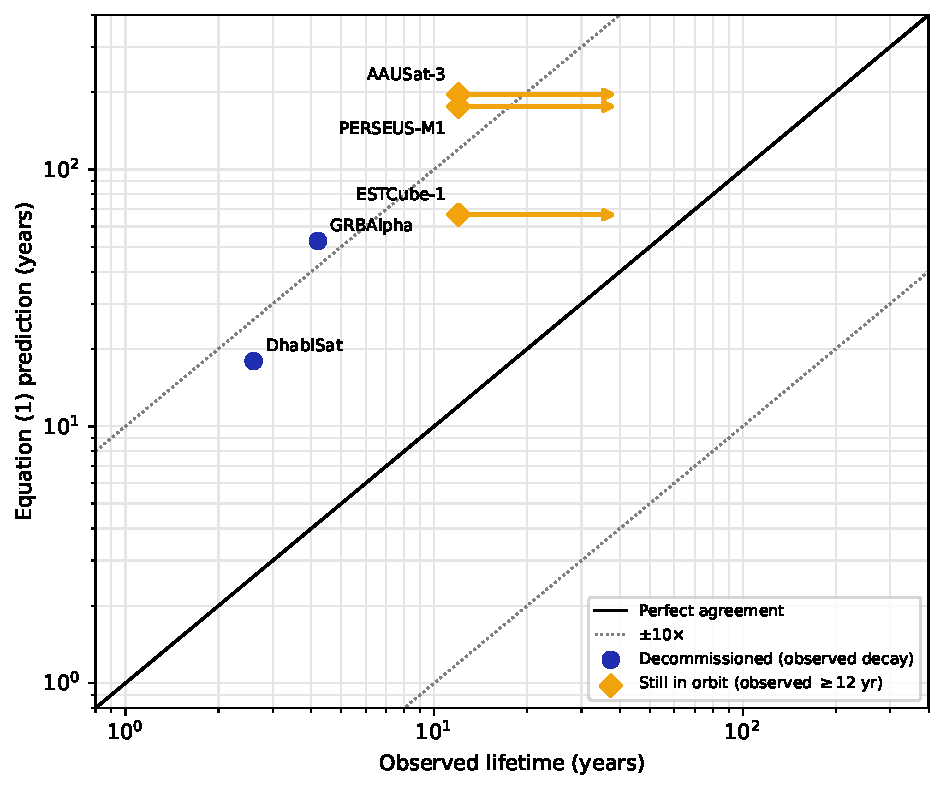
\includegraphics[width=0.62\linewidth]{figures/fig_validation.pdf}
\caption{Equation~(\ref{eq:decay}) predictions versus observed lifetimes. Blue circles: CubeSats that have decayed. Orange diamonds with arrows: satellites still in orbit after 12+ years (observed lifetime is a lower bound). The solid line is perfect agreement; dotted lines mark a factor of ten.}
\label{fig:resid}
\end{figure}

The model overestimates the lifetime of both decayed satellites, by a factor of \ValLo{} to \ValHi{}. The predictions for the three satellites still in orbit (\ValEstFour{}, \ValAauThree{} and \ValPerseus{} years) are consistent with their continued presence in orbit, but this is only a lower-bound check. These results show that the model is not an accurate absolute predictor for the decayed satellites tested here (initial altitudes of about 400--550\,km): the single exponential with $H=100$\,km does not capture the steeper density decline of the real atmosphere or its variation with solar activity. The model is therefore used in this paper for its \emph{relative} ranking of technologies, which is independent of $K$ and $H$ because all three systems are evaluated at the same altitude and differ only in $A/m$ (the ratio of two deorbit times equals the inverse ratio of their $A/m$ values). Absolute times, and in particular statements about whether a passive electrodynamic tether or a propulsion system meets the 25-year guideline, should be treated as model-dependent and confirmed with a higher-fidelity tool before being relied upon.

\section{Results}
\subsection{Model Validation and Predictive Accuracy}
Validation against five CubeSats (Table~\ref{tab:val}, Figure~\ref{fig:resid}) shows that the model overestimates the observed lifetimes of the two decayed satellites by a factor of \ValLo{} to \ValHi{}. The predictions for the three satellites that remain in orbit are consistent with their persistence. The model is consequently best interpreted as a tool for comparing technologies against one another rather than for predicting absolute lifetimes (Section~\ref{sec:val}).

\subsection{Deorbit Performance Across Altitudes}
The calculated deorbit times for the three technologies revealed significant performance differences across the 400--800\,km altitude range (Table~\ref{tab:times}). Deorbit time exhibited strong exponential sensitivity to initial altitude for all systems, as visualized in the semi-logarithmic plot in Figure~\ref{fig:alt}.

\begin{table}[H]
\centering
\caption{Calculated deorbit times (years) from various initial altitudes.}
\label{tab:times}
\begin{tabular}{rrrr}
\toprule
Altitude (km) & Drag Sail & E.D.\ Tether & Propulsion \\
\midrule
400 & 0.3 & 6.1 & 23.7 \\
500 & 0.8 & 16.7 & 64.3 \\
600 & 2.2 & 45.4 & 174.8 \\
700 & 5.9 & 123.4 & 475.2 \\
800 & 16.0 & 335.4 & 1291.7 \\
\bottomrule
\end{tabular}
\end{table}


\begin{figure}[H]
\centering
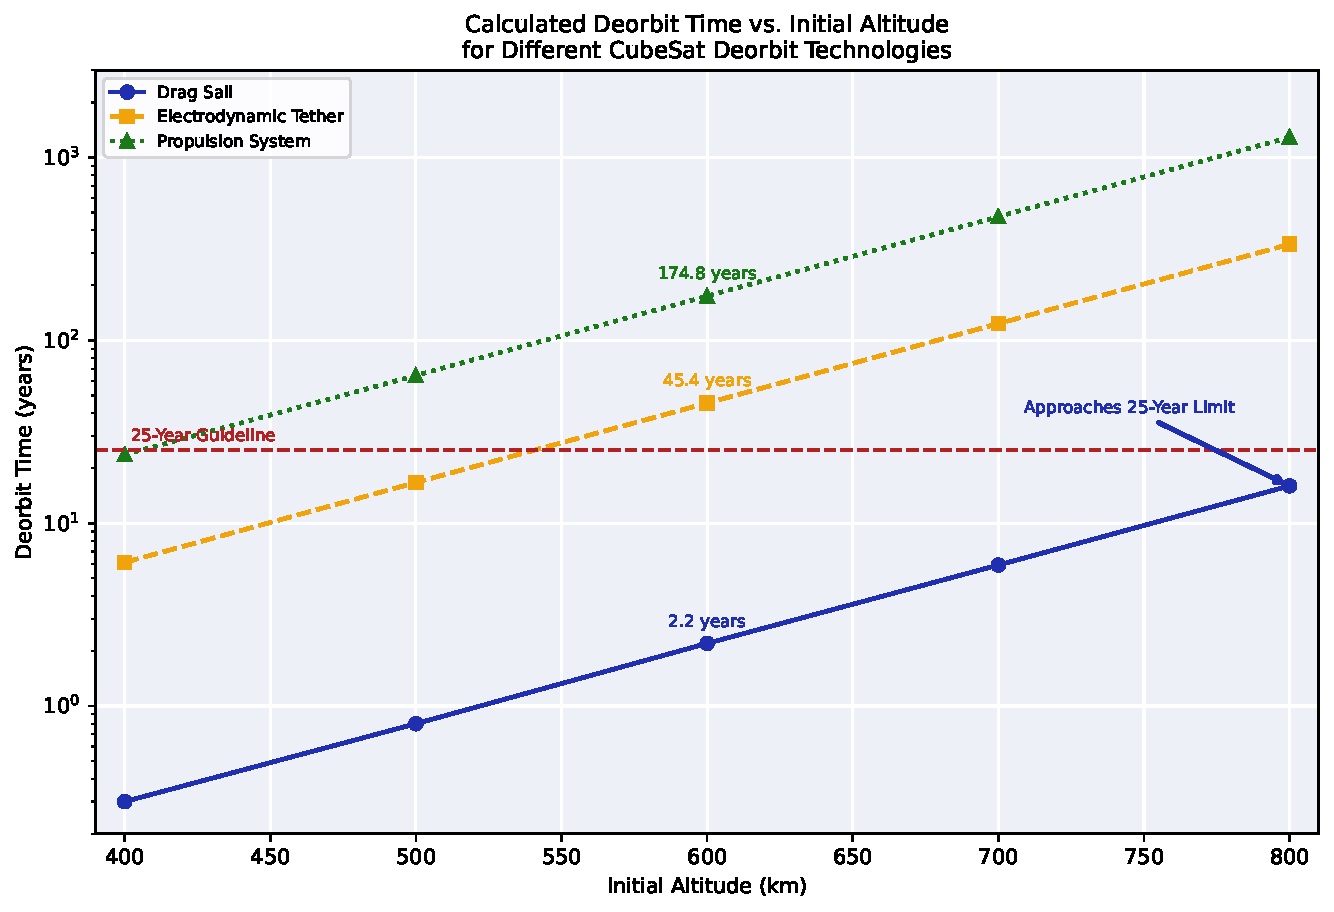
\includegraphics[width=0.85\linewidth]{figures/fig_deorbit_vs_altitude.pdf}
\caption{Calculated deorbit time versus initial altitude for CubeSat deorbit technologies. Semi-logarithmic plot of deorbit time (years) as a function of initial altitude (km). The drag sail (solid blue line) demonstrates the shortest deorbit times across all altitudes, while the propulsion system (dotted green line) exhibits the longest. The 25-year guideline is shown as a dashed red horizontal line. The electrodynamic tether (dashed orange line) exceeds the guideline above approximately \EDTcross\,km, and the propulsion system above approximately \PROPcross\,km.}
\label{fig:alt}
\end{figure}

The drag sail was the only technology that complied with the 25-year rule across the entire altitude range studied, deorbiting in approximately \SailSix{} years from a standard 600\,km altitude. In contrast, the passively modeled electrodynamic tether and the propulsion system exceeded the guideline at 600\,km by \EDTover\% and \PROPover\%, respectively, within the limits of the model's absolute accuracy (Section~\ref{sec:val}).

\subsection{Determinants of Deorbit Performance}
The fundamental parameter governing deorbit performance was the effective area-to-mass ratio ($A/m$). Figure~\ref{fig:am} illustrates the strong inverse correlation between the $A/m$ ratio and the deorbit time at a 600\,km altitude.

\begin{figure}[H]
\centering
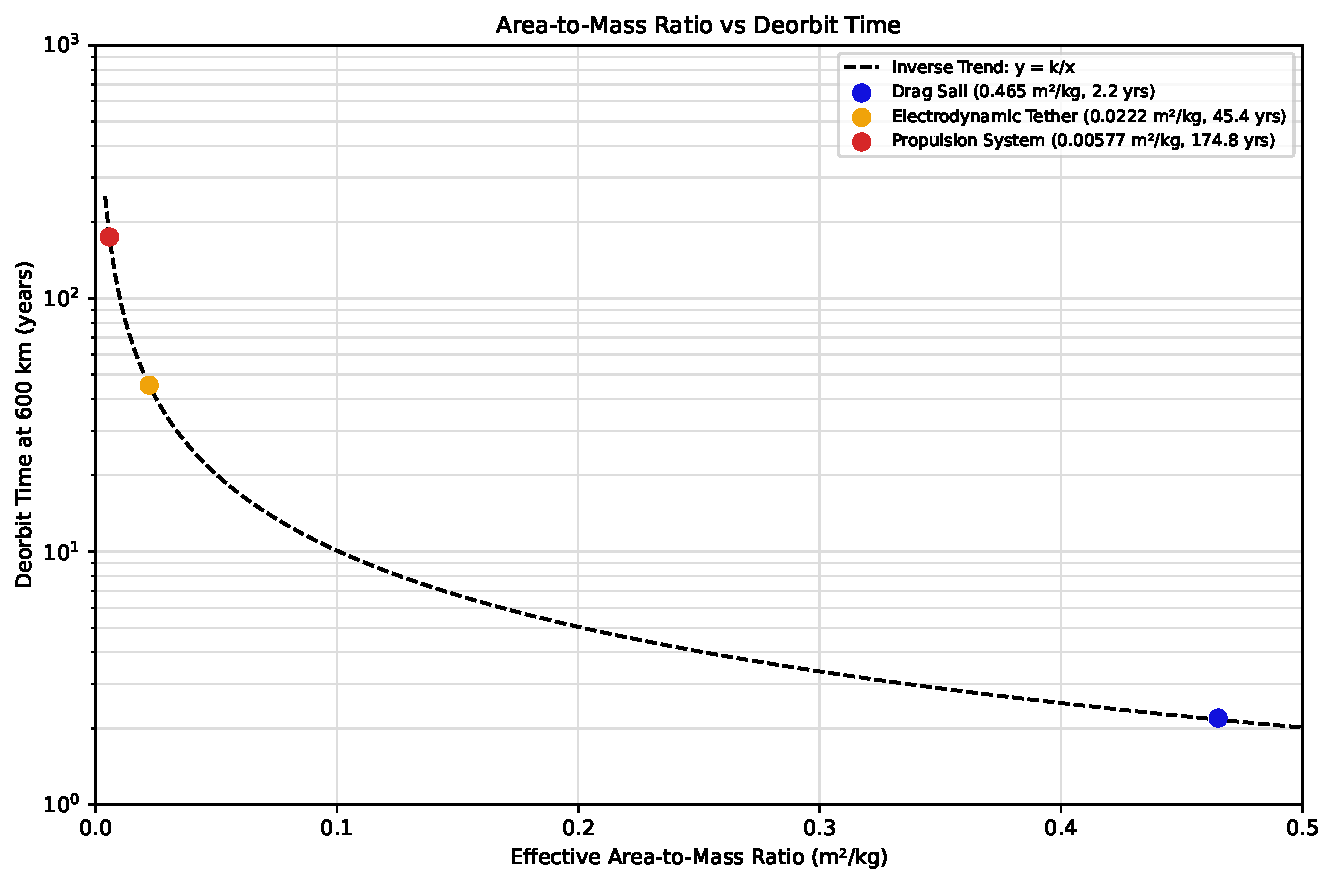
\includegraphics[width=0.8\linewidth]{figures/fig_am_vs_time.pdf}
\caption{Area-to-mass ratio versus deorbit time at 600\,km altitude. The drag sail ($A/m = 0.465$\,m$^2$/kg) achieves rapid deorbit in \SailSix{} years, while the electrodynamic tether ($0.0222$\,m$^2$/kg) requires \EDTSix{} years, and the propulsion system ($0.00577$\,m$^2$/kg) exhibits the longest decay time of \PropSix{} years. The inverse trend line ($y = k/x$) highlights the strong negative correlation.}
\label{fig:am}
\end{figure}

A direct performance comparison at the standard 600\,km altitude (Figure~\ref{fig:bar}) shows how each technology compares with the 25-year guideline. Only one of the three technologies (the drag sail) falls below it in the model, underscoring the importance of technology selection for space debris mitigation.

\begin{figure}[H]
\centering
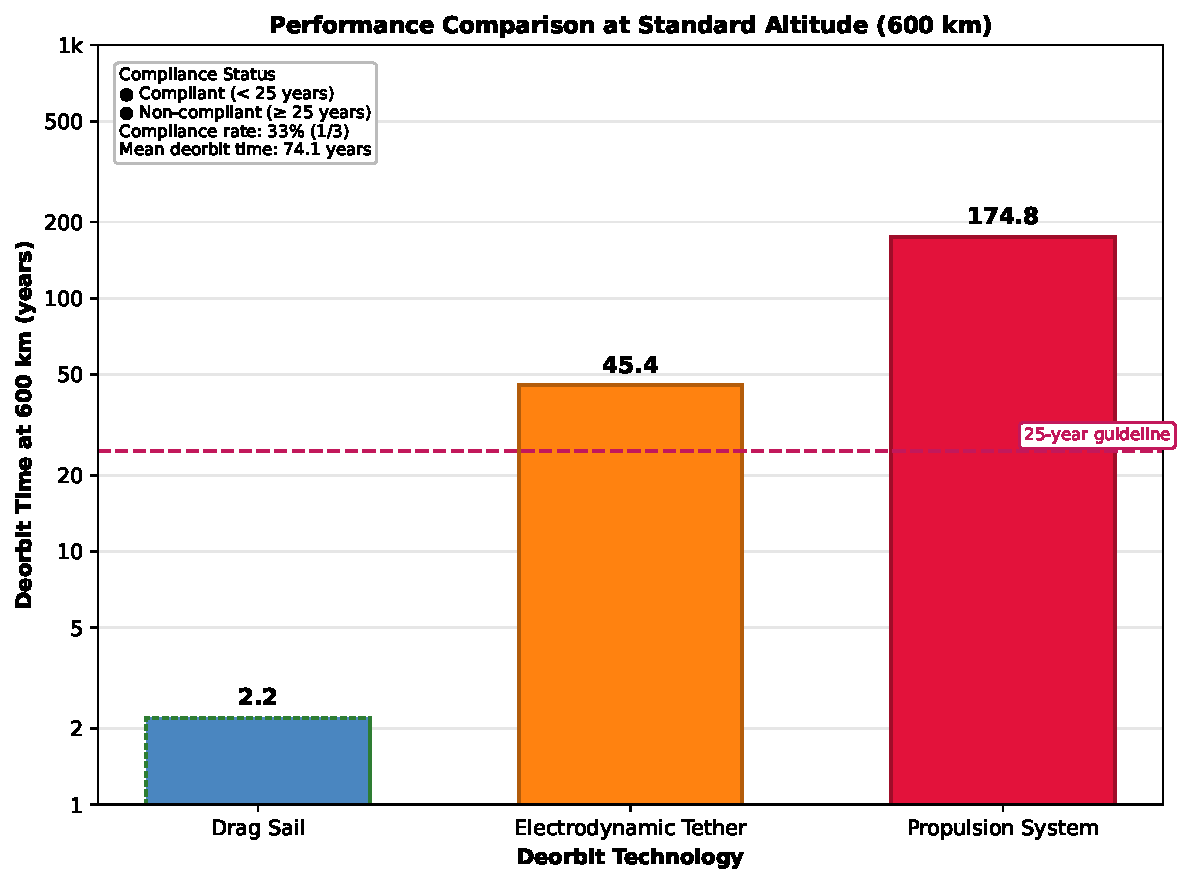
\includegraphics[width=0.75\linewidth]{figures/fig_performance_600km.pdf}
\caption{Performance comparison of deorbit technologies at 600\,km altitude. The drag sail (\SailSix{} years) provides a substantial margin below the 25-year guideline. Both the electrodynamic tether (\EDTSix{} years) and the propulsion system (\PropSix{} years) exceed the limit. The logarithmic scale accommodates the orders-of-magnitude difference in performance.}
\label{fig:bar}
\end{figure}

\section{Discussion}
\subsection{Interpretation of Findings and Hypothesis Evaluation}
Our quantitative results support the performance part of our initial hypothesis: in the model, a drag sail gives the shortest passive deorbit time and is the only one of the three options that meets the 25-year deorbit guideline for a typical CubeSat in Low Earth Orbit (LEO). The cost and reliability parts of the hypothesis were not modeled and remain untested here. The data show that a 3U CubeSat equipped with a drag sail deorbits in approximately \SailSix{} years from a standard altitude of 600\,km. This timeframe is well inside the 25-year guideline. It reflects passive decay performance only and says nothing about the reliability of sail deployment, which is a separate failure mode.

This high performance is a direct result of the drag sail's fundamental operating principle: it significantly increases the satellite's effective area-to-mass ratio ($A/m$). With an $A/m$ of 0.465\,m$^2$/kg, the satellite experiences maximum atmospheric drag force for its mass. The versatility of this technology is clear across the operational altitude range for CubeSats; it provides rapid deorbit times of \SailFour{} years at 400\,km and still complies with the 25-year rule even at 800\,km, with a calculated deorbit time of \SailEight{} years.

Our comparative analysis reveals critical trade-offs between the three deorbit technologies, offering nuanced insights beyond a simple performance ranking.

\paragraph{Electrodynamic Tethers (EDTs): the implications of conservative modeling.} The calculated deorbit time of \EDTSix{} years for the EDT at 600\,km is a direct outcome of our deliberate choice to model it as a passive device based solely on its physical cross-section. This result should be interpreted as a conservative baseline that illustrates a crucial failure mode, rather than as a representation of the technology's full potential. A fully functional EDT operates on an active principle, generating a decelerating Lorentz force by driving an electrical current through a long conductive tether as it moves through Earth's magnetic field. Literature confirms that operational EDTs can achieve deorbit from altitudes as high as 800\,km in less than a year, and in a matter of weeks from lower altitudes~\cite{bilen,sarego,nasa2021}.

The primary challenge for EDTs, therefore, lies not in their theoretical performance but in their technical reliability and operational complexity. Successful deorbit requires the flawless deployment of a long, fragile tether, the maintenance of a stable electrical connection with the ionospheric plasma, and the mitigation of dynamic instabilities ~\cite{sanchez,nasa2021}. While our model ranks EDTs poorly under passive assumptions, they remain a uniquely valuable technology for active deorbiting from very high altitudes where atmospheric drag is minimal. The extended deorbit time in our results serves as a critical warning: a failure of the active electrodynamic systems would leave the satellite in orbit for decades due to the tether's negligible contribution to passive drag.

\paragraph{Propulsion systems: the resource trade-off for active control.} When modeled without an active deorbit burn---considering only its contribution to passive decay---a CubeSat with a cold-gas propulsion system exhibited the longest deorbit time of \PropSix{} years at 600\,km. This demonstrates that propulsion systems are ineffective for passive orbital decay.

Their value is unlocked only when used for active, controlled deorbit maneuvers or for orbital maintenance. For missions where a propulsion system is already a core requirement for primary objectives (such as orbital adjustments or formation flying), it can efficiently serve a dual purpose for end-of-life disposal. However, incorporating a propulsion system solely for the purpose of deorbit represents the most mass-inefficient and cost-inefficient approach, as clearly reflected in its very low $A/m$ ratio of 0.00577\,m$^2$/kg.

These findings collectively illustrate that for the majority of CubeSat missions, particularly those developed by universities and small satellite teams where simplicity is paramount, integrating a drag sail from the initial design phase offers the passive approach with the shortest modeled deorbit time, subject to the reliability of its deployment mechanism, which this study does not model.

\subsection{Comparison with Existing Literature}
Our study provides a quantitative foundation that reinforces and extends conclusions from prior research. Earlier reviews and technology surveys have qualitatively described drag sails as a ``mature and cost-effective'' deorbit solution ~\cite{visagie,altaf}; our work substantiates these claims by supplying concrete deorbit timelines across a range of altitudes, from 400\,km to 800\,km. Similarly, while the high potential performance and the associated deployment and reliability challenges of electrodynamic tethers have been noted in the literature ~\cite{sanchez,sarego}, our analysis establishes a concrete numerical baseline for the consequences of system failure, quantifying the risk of extended orbital lifetime. The resource-intensive nature of propulsion systems for small satellites is well-documented ~\cite{lemmer,selva}; here, we have quantified the dramatic impact that a low $A/m$ ratio has on passive decay timelines, underscoring why propulsion is not a set-and-forget solution.

By applying a unified modeling approach and consistent assumptions, this study translates these previously qualitative technology assessments into directly comparable, measurable deorbit timelines. This provides the CubeSat community with actionable, data-driven guidance for technology selection during the critical mission planning phase.

\subsection{Limitations of the Study and Sensitivity Analysis}
While our model provides a valuable first-order framework for comparison, it is essential to acknowledge its simplifying assumptions and their potential impact.

\paragraph{Solar activity variations.} The 11-year solar cycle causes significant fluctuations in solar extreme ultraviolet (EUV) radiation, which heats the upper atmosphere and dramatically alters its density. This natural variation can change actual deorbit times by a factor of 10 or more between solar minimum and maximum conditions. Our model, calibrated to historical average data, does not capture this temporal variability.

\paragraph{Satellite attitude dynamics.} We assumed a constant, maximum cross-sectional area oriented optimally into the velocity vector. In reality, a tumbling or non-optimally oriented satellite would present a smaller effective area, reducing drag and potentially increasing deorbit times.

\paragraph{Orbital eccentricity.} The analysis was conducted for circular orbits. Satellites in elliptical orbits experience highly variable drag forces, with most of the decay occurring at perigee, requiring more complex modeling for accurate lifetime predictions.

\paragraph{Electrodynamic tether modeling.} As previously emphasized, the most significant simplification in our study concerns the EDT, which was modeled exclusively for its passive drag contribution. A comprehensive model of an operational EDT would require complex, coupled analysis of the space plasma environment, tether current collection physics, and geomagnetic field interactions ~\cite{bilen,sarego,nasa2021}. Our results for the EDT must be viewed as a conservative lower-bound estimate of its performance.

\paragraph{Model bias.} As shown in Section~\ref{sec:val}, Equation~(\ref{eq:decay}) overestimates the lifetimes of satellites that have already decayed by a factor of \ValLo--\ValHi. If a similar bias applies at 600\,km, the absolute times for the electrodynamic tether and the propulsion system could be considerably shorter than those in Table~\ref{tab:times}, and their non-compliance with the 25-year guideline would not be established by this model alone. The drag-sail result (compliant at every altitude) would only improve, and the ranking of the technologies is unaffected.

\paragraph{Quantitative sensitivity analysis.} To evaluate the robustness of our conclusions against these limitations, we performed a sensitivity analysis on key model parameters at 600\,km. A $\pm50\%$ variation in atmospheric density (simulating extreme solar activity) changed the drag-sail deorbit time between \DensLo{} and \DensHi{} years, a spread of about a factor of three between the extremes. However, it did not alter the fundamental performance hierarchy; drag sails remained the fastest deorbit option across all scenarios. Similarly, a 10\% uncertainty in the effective area-to-mass ratio (plausible due to attitude variations or deployment anomalies) resulted in approximately 9--11\% changes in deorbit times. A 15\% variation in the empirical constant $K$ (reflecting model calibration uncertainty) changed the deorbit time at 600\,km by $\pm\KsensSail$ years for the drag sail, $\pm\KsensEDT$ years for the electrodynamic tether and $\pm\KsensProp$ years for the propulsion system. Crucially, across all tested scenarios, drag sails consistently maintained compliance with the 25-year guideline at 600\,km, while the other technologies failed to do so. This confirms that the ranking of the technologies and the drag-sail result are robust to these parameter variations; the validation bias described above is, however, larger than the perturbations tested here, so the non-compliance of the other two technologies is model-dependent.

\subsection{Implications and Future Research}
The quantitative framework developed in this study empowers CubeSat developers with a practical, data-driven tool for deorbit technology selection. For the vast majority of educational and commercial missions targeting altitudes below 700\,km, our analysis indicates that a drag sail is the passive option with the shortest modeled deorbit time and a promising route to meeting the 25-year guideline, pending assessment of deployment reliability and regulatory requirements, which this study does not address.

Future research should build upon this foundation to address its limitations and explore advanced concepts:
\begin{enumerate}
\item \textbf{Advanced Electrodynamic Tether Modeling:} Developing a more sophisticated model that incorporates the active Lorentz force mechanism would enable a direct and fair comparison of the operational performance of all three technologies.
\item \textbf{Solar Activity Integration:} Creating a model that can incorporate real-time or forecasted solar flux data would allow for mission-specific decay predictions that account for the phase of the solar cycle, greatly enhancing predictive accuracy for operational planning.
\item \textbf{Hybrid System Evaluation:} Investigating the performance and trade-offs of hybrid systems---such as a combined drag sail and electrodynamic tether, or a drag sail with a miniature propulsion module---could identify optimal solutions for challenging orbital regimes, particularly very high altitudes or missions requiring precise deorbit control.
\end{enumerate}
In summary, this study moves the discussion on CubeSat end-of-life disposal from qualitative descriptions to a quantitative, comparative framework. It provides student researchers and small satellite developers with the necessary insights to make informed, responsible design choices that support the long-term sustainability of the low-Earth orbit environment.

\section{Conclusion}
This study establishes a practical, first-order comparative framework for evaluating deorbit technologies for CubeSats and quantifies its limitations against observed satellite lifetimes. Our analysis demonstrates that for the majority of low-Earth orbit missions, passive drag sails give the shortest modeled deorbit time and are the only one of the three technologies that the model places within the 25-year guideline across 400--800\,km. Reliability, cost and regulatory acceptance were not modeled. The sensitivity analysis confirms that this central finding holds across a range of expected environmental and model parameter variations, thereby giving CubeSat developers greater confidence in the relative ranking of the technologies. Absolute deorbit times from this simplified model should be treated as upper estimates and verified with a higher-fidelity tool during detailed design.

The implications of this work extend to multiple stakeholders in the small satellite community. Educational institutions can integrate this straightforward model into spacecraft design curricula to teach orbital mechanics and space sustainability principles. Small satellite teams can use it to perform rapid, preliminary technology trade-offs during the proposal and early design stages. Furthermore, regulatory bodies may consider the adoption of such simplified, transparent models for the compliance verification of university-class CubeSat projects.

The methodology presented here also opens several avenues for future work. These include the integration of real-time solar activity data to generate mission-specific decay predictions, and the extension of the model to higher altitude regimes where different technologies, such as electrodynamic tethers, may become optimal. Most immediately, this framework empowers the rapidly growing CubeSat community to transform deorbit system selection from a theoretical challenge into a straightforward, actionable, and responsible design choice.

\nocite{forshaw,biddy}
\begin{thebibliography}{99}\small
\bibitem{villela} T.~Villela et al.\ (2019). Towards the thousandth CubeSat: A statistical overview. \emph{International Journal of Aerospace Engineering}, 2019, Article 5063145. doi:10.1155/2019/5063145
\bibitem{esa2025} European Space Agency, Space Debris Office (2025). \emph{ESA Space Environment Report 2025}, 1 April 2025. https://www.esa.int/Space\_Safety/Space\_Debris/ESA\_Space\_Environment\_Report\_2025
\bibitem{kessler} D.~J. Kessler and B.~G. Cour-Palais (1978). Collision frequency of artificial satellites: The creation of a debris belt. \emph{J.\ Geophys.\ Res.\ Space Phys.}, 83(A6), 2637--2646. doi:10.1029/JA083iA06p02637
\bibitem{iadc} Inter-Agency Space Debris Coordination Committee (IADC) (2021). IADC Space Debris Mitigation Guidelines, IADC-02-01.
\bibitem{lemmer} K.~Lemmer (2017). Propulsion for CubeSats. \emph{Acta Astronautica}, 134, 231--243. doi:10.1016/j.actaastro.2017.01.048
\bibitem{selva} D.~Selva and D.~Krejci (2019). A comparative analysis of CubeSat propulsion technologies. \emph{Acta Astronautica}, 155, 308--319. doi:10.1016/j.actaastro.2018.08.031
\bibitem{sanchez} G.~Sanchez-Arriaga, J.~R. Sanmartin and E.~C. Lorenzini (2017). Comparison of technologies for deorbiting spacecraft from low-Earth orbit at end of mission. \emph{Acta Astronautica}, 138, 536--542. doi:10.1016/j.actaastro.2017.01.018
\bibitem{altaf} A.~Altaf et al.\ (2023). A comprehensive review of deorbiting mechanisms for small satellites. \emph{Progress in Aerospace Sciences}, 141, 100922. doi:10.1016/j.paerosci.2023.100922
\bibitem{zhang} R.~Zhang and Y.~He (2024). Overview and key technology of the membrane drag sail for LEO deorbiting. \emph{Space Science \& Technology}, 40(2), 145--160. doi:10.34133/space.0115
\bibitem{chen} J.~Chen, S.~Chen, Y.~Qin, Z.~Zhu and J.~Zhang (2024). Aerodynamic analysis of deorbit drag sail for CubeSat using DSMC method. \emph{Aerospace}, 11(4), 315. doi:10.3390/aerospace11040315
\bibitem{forward} R.~L. Forward and R.~P. Hoyt (1999). Terminator Tether: A spacecraft deorbit device. \emph{J.\ Spacecraft and Rockets}, 36(2), 187--196. doi:10.2514/2.3446
\bibitem{ohkawa} Y.~Ohkawa et al.\ (2012). Electrodynamic tether propulsion for orbital debris deorbit. \emph{J.\ Space Technology and Science}, 26(1), 33--46. doi:10.11230/jsts.26.1\_33
\bibitem{sarego} G.~Sarego et al.\ (2020). Deorbiting performance of electrodynamic tethers to mitigate space debris. \emph{Acta Astronautica}, 168, 62--74. doi:10.1016/j.actaastro.2020.06.014
\bibitem{nasa2022} NASA (2022). Technology taxonomy for end-of-mission disposal of small spacecraft (NASA/TP-2022-0018058).
\bibitem{bilen} S.~G. Bil\'en (2021). Space tethers demonstrate deorbit capability. \emph{Aerospace America} (AIAA), 2021. https://aerospaceamerica.aiaa.org/year-in-review/space-tethers-demonstrate-deorbit-capability/
\bibitem{nasa2021} NASA (2021). State-of-the-art of electrodynamic tether technology for deorbiting small spacecraft (NASA/TP-2021-021263).
\bibitem{visagie} L.~Visagie et al.\ (2015). Comparison of passive de-orbiting systems for CubeSat and design of a drag-sail device. \emph{Proc.\ 66th International Astronautical Congress (IAC)}.
\bibitem{forshaw} J.~L. Forshaw et al.\ (2016). RemoveDEBRIS: An in-orbit demonstration of space debris removal technologies. \emph{Acta Astronautica}, 127, 448--463. doi:10.1016/j.actaastro.2016.06.018
\bibitem{biddy} C.~Biddy and T.~Svitek (2012). LightSail-1: A solar sailing demonstration mission. \emph{Proc.\ 26th AIAA/USU Conference on Small Satellites}, SSC12-I-1.
\end{thebibliography}

\end{document}
